\chapter{Συγγραφή – Κείμενο – Λοιπά στοιχεία}\label{chap:writing}
\chapterauthor{Κεντρική Ομάδα Υποστήριξης}[Κεντρική Ομάδα Υποστήριξης\\  Κάλλιπος, Ανοικτές Ακαδημαϊκές Εκδόσεις]

\section{Ροή εργασίας}
Το διάγραμμα που ακολουθεί απεικονίζει την προτεινόμενη ροή εργασίας για τη συγγραφή
και τελική παράδοση ενός βιβλίου στο πλαίσιο του Έργου ΚΑΛΛΙΠΟΣ+.

\begin{figure} \centering
\renewcommand{\figurename}{Σχήμα}
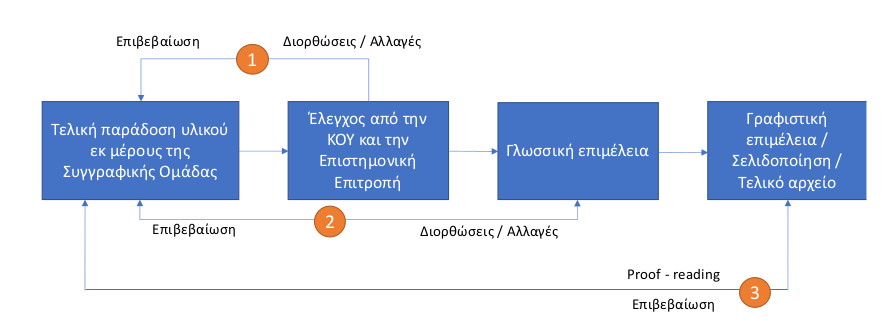
\includegraphics[width=0.8\textwidth]{images/work_flow.png}
\caption[Ροή εργασίας.]{Ροή εργασίας μετά την παράδοση του υλικού εκ μέρους
της Συγγραφικής Ομάδας.}
\label{fig:work_flow}
\end{figure}

Η Συγγραφική Ομάδα οφείλει -στο τέλος του χρονοδιαγράμματος του Έργου- να
παραδώσει το σύνολο του υλικού σύμφωνα με τις προδιαγραφές που καταγράφονται στο
Κεφάλαιο \ref{chap:best-practice}. Στη συνέχεια, η ΚΟΥ και η Επιστημονική Επιτροπή (ΕΕΣΑ) του Έργου (με
τη βοήθεια των Αξιολογητών) θα προβαίνουν στον έλεγχο του υλικού σε επίπεδο τεχνικής
αρτιότητας και επιστημονικής επάρκειας (αντίστοιχα). Τυχόν υποδείξεις για αλλαγές -
διορθώσεις λαθών κλπ. θα αποστέλλονται προς τη Συγγραφική Ομάδα (Βήμα 1). Εφόσον
ολοκληρωθεί με επιτυχία ο έλεγχος του 1ου βήματος, το υλικό θα παραδίδεται σε ειδικό
γλωσσικό επιμελητή. Ο γλωσσικός επιμελητής θα συνεργάζεται στενά με τα μέλη της
Συγγραφικής Ομάδας για διορθώσεις και προσαρμογές (Βήμα 2). Στο τελικό στάδιο, και
αμέσως μετά τη διαδικασία της γλωσσικής επιμέλειας, το υλικό θα παραδίδεται σε ειδικό
ψηφιακό στοιχειοθέτη / γραφίστα για τη σελιδοποίηση και την παραγωγή των τελικών
δοκιμίων του βιβλίου (τόσο σε ηλεκτρονική μορφή όσο και σε τυπογραφικά δοκίμια). Όπως
και στα προηγούμενα στάδια, έτσι και σ’ αυτό το στάδιο ο τελικός έλεγχος θα
πραγματοποιείται από τη Συγγραφική Ομάδα και την ΚΟΥ, από την οποία θα παρέχεται
και η έγκριση για τη δημοσίευση/ανάρτηση του έργου στο Αποθετήριο ΚΑΛΛΙΠΟΣ.
Παρόμοια διαδικασία θα ακολουθείται για την ενδιάμεση παράδοση / παραλαβή υλικού
από τις Συγγραφικές Ομάδες. Ειδικότερα, σε ό, τι αφορά την Ενδιάμεση Αναφορά, η ΚΟΥ
θα προβαίνει σε έλεγχο του συγγραφικού υλικού, σε επίπεδο τεχνικής αρτιότητας, και, σε
συνεργασία με τα μέλη της Επιστημονικής Επιτροπής θα ελέγχει την επιστημονική
επάρκεια, καθώς και το αν τηρούνται οι επιπλέον όροι που τυχόν τέθηκαν κατά το στάδιο
της Αξιολόγησης των Προτάσεων συγγραφής.

Εφόσον οι έλεγχοι του Παραδοτέου υλικού, τόσο κατά την Τελική, όσο και κατά την
Ενδιάμεση Παράδοση/Αναφορά, αξιολογηθούν θετικά, τότε θα αποδεσμεύονται και τα
αντίστοιχα χρηματικά ποσά για την αποζημίωση και των μελών των Συγγραφικών Ομάδων
και των λοιπών Συντελεστών επικουρικών εργασιών.

\section{Δομή – Μορφή κειμένου}
Το κείμενο θα πρέπει να ακολουθεί συγκεκριμένη δομή και μορφή, σύμφωνα με τις
οδηγίες του παρόντος εγγράφου. Η χρήση άλλων εργαλείων
συγγραφής (πχ. LaTeX/XeLaTeX, DocBook) είναι δυνατή μετά από συνεννόηση με την
KOY. Επιπλέον, ο βασικός μορφότυπος για την ανάρτηση και προβολή της ηλεκτρονικής
μορφής του βιβλίου στο Αποθετήριο ΚΑΛΛΙΠΟΣ είναι το PDF.

Εφόσον οι Συγγραφείς έχουν ήδη ολοκληρώσει τη συγγραφή, τότε και μόνο τότε
μπορούν να το παραδώσουν ως έχει, φροντίζοντας απλώς να το συμμορφώσουν, πριν
την παράδοση, στις υποδείξεις που παρέχονται στον παρόντα Οδηγό όσον αφορά την
ονοματοδοσία και δομή των αρχείων (βλ. Κεφάλαιο \ref{chap:best-practice}), τα μεταδεδομένα κλπ.

\subsection{Γενικές οδηγίες διαμόρφωσης και οργάνωσης του κειμένου}
Οι επόμενες οδηγίες θα εφαρμόζονται σε όλα τα πρότυπα αρχεία του κειμένου (πρώτες
σελίδες, περιεχόμενα, εισαγωγή, πρόλογος, κεφάλαια κλπ.):
\begin{itemize}
\item Μορφότυπος (format) αρχείων κειμένου: αρχεία tex
\item Μέγεθος σελίδας: υποχρεωτικά $205\times297$mm. Προαιρετικά για τυπογραφική εκτύπωση $170\times240$mm
\item Περιθώρια: είναι καθορισμένα από το εκάστοτε πρότυπο συγγραφής
\item Διαστήματα: είναι καθορισμένα από το εκάστοτε πρότυπο συγγραφής
\item Γραμματοσειρά (είδος, μέγεθος): arimo (ttf), arno-pro(otf) 11 pt (σε κυρίως κείμενο), 10 pt (σε υποσημειώσεις, λεζάντες).
\item Συλλαβισμός: το κείμενο θα έχει συλλαβισμό
\item Κεφαλίδες, υποσέλιδα: είναι καθορισμένα από το εκάστοτε πρότυπο συγγραφής
\item Σελιδαρίθμηση: είναι καθορισμένη από το εκάστοτε πρότυπο συγγραφής
\item Αρίθμηση-Λεζάντες: Οι λεζάντες των Σχημάτων/Εικόνων κλπ. θα περιέχουν και την
αντίστοιχη αρίθμησή τους. Οι λεζάντες θα γράφονται με τον εξής τρόπο: <Τίτλος λεζάντας
\_αριθμός κεφαλαίου. αριθμός Σχήματος/Εικόνας\_κείμενο λεζάντας>. Οι λεζάντες θα
καταλήγουν σε τελεία (βλ. για παράδειγμα τη λεζάντα στο Σχήμα 2.1 παραπάνω). Τέλος,
συστήνεται να τοποθετούνται κάτω από την Εικόνα, το Σχήμα ή το πολυμεσικό
αντικείμενο και κάτω ή επάνω (προτιμητέο) από τον Πίνακα.
\item Οι μαθηματικοί τύποι και οι χημικές αντιδράσεις μπορούν να γραφούν με την χρήση
των αντίστοιχων πακέτων του \LaTeX / \XeLaTeX\ (Πχ. για χημικές αντιδράσεις chemfig,
mhchem, chemformula κά.).
\item Υπερσύνδεσμοι: Είναι δυνατή η προσθήκη υπερσυνδέσμων (links) σε τοποθεσίες του
διαδικτύου στις οποίες μπορεί να φιλοξενείται περιεχόμενο σχετικό με το σύγγραμμα. Η
ευθύνη διατήρησης του περιεχομένου, ώστε οι υπερσύνδεσμοι να μην παύουν να ισχύουν
(broken links), είναι ευθύνη του Συγγραφέα. Σημειώνεται ότι, αν το URL του συνδέσμου
είναι μεγάλο, δεν είναι απαραίτητο να ενσωματώνεται στο κείμενο, αφού επιτρέπεται να
είναι διαφορετικό το κείμενο του υπερσυνδέσμου από το URL στο οποίο παραπέμπει.
\item Ειδικά σύμβολα: Ιδιαίτερη προσοχή απαιτείται στη χρήση συμβόλων. Για τα ειδικά σύμβολα
που χρησιμοποιούνται στο \LaTeX / \XeLaTeX\ μπορείτε να ανατρέξετε στον υπερσύνδεσμο
\url{https://latex.wikia.org/wiki/List_of_LaTeX_symbols}.
\end{itemize}

\section{Άλλα στοιχεία}

\begin{itemize}
\item Πίνακες: οι Πίνακες δεν πρέπει να έχουν εφέ (effects). Για τη διαμόρφωση των Πινάκων
βλ. παράγραφο \ref{subsec:tables}.
\item Εμφάνιση πολυμεσικών-διαδραστικών αντικειμένων και συνδέσμων (links) εκτός
σύνδεσης δικτύου (offline): Στις περιπτώσεις που δεν είναι δυνατή η σύνδεση σε δίκτυο,
ώστε να είναι ενεργοί οι σύνδεσμοι, απαιτείται περιγραφή του πολυμεσικού/διαδραστικού
αντικειμένου ή του συνδέσμου μέσα στο κείμενο. Γι’ αυτόν τον λόγο, όπου οι συγγραφείς
το κρίνουν απαραίτητο θα γίνεται εισαγωγή (εντός του κειμένου) Πίνακα (με την ακόλουθη
διαμόρφωση) όπου και θα αναφέρονται τα εξής:
\begin{itemize}
\item Τίτλος αντικειμένου/συνδέσμου
\item Τύπος υλικού (πχ. ηχητικό απόσπασμα)
\item Περιγραφή αντικειμένου/συνδέσμου
\end{itemize}
\end{itemize}

\subsection{Περιεχόμενα}

Το βάθος του επιπέδου περιεχομένων δεν πρέπει να ξεπερνά το τέταρτο επίπεδο.

\subsection{Πίνακας Συντομεύσεων-Ακρωνυμίων}

Μετά τα περιεχόμενα θα πρέπει να ακολουθεί Πίνακας (ή Πίνακες) με τις
ελληνόγλωσσες και ξενόγλωσσες συντομεύσεις (ακρωνύμια) που χρησιμοποιούνται στο
κείμενο.

\subsection{Βιβλιογραφία-Αναφορές-Υποσημειώσεις}

Σχετικά με την παρεχόμενη Βιβλιογραφία, ανάλογα με τη συνήθη πρακτική του
επιστημονικού τομέα, οι Συγγραφείς μπορούν να ενσωματώνουν Αναφορές ή
Βιβλιογραφία στο τέλος του κάθε Κεφαλαίου (προτιμητέο, εφόσον κάθε Κεφάλαιο
συνιστά αυτόνομο μαθησιακό αντικείμενο) ή/και συγκεντρωτικά στο τέλος βιβλίου.
Στη Βιβλιογραφία μπορούν να περιλαμβάνονται και αναφορές σε ιστοσελίδες
(δικτυογραφία). Είναι επιθυμητό το να παρέχεται, όπου είναι δυνατό, και το αναγνωριστικό
του αντικειμένου στο οποίο γίνεται αναφορά, για παράδειγμα το DOI για άρθρα σε
περιοδικά, το ISBN για βιβλία κλπ.

Η μορφοποίηση των Αναφορών πρέπει να είναι ομοιόμορφη σε όλο το σύγγραμμα.
Μπορεί να ακολουθεί τη μορφοποίηση της IEEE (χωρίς τις συντομεύσεις απαραίτητα),
προκειμένου για συγγράμματα στις Επιστήμες Μηχανικών κλπ. ή ένα από τα βιβλιογραφικά
συστήματα APA, MLA, Chicago κλπ., προκειμένου για συγγράμματα Ανθρωπιστικών και
Κοινωνικών Επιστημών (πάντως είναι αποδεκτό και οποιαδήποτε άλλο σύστημα,
προφανώς συμβατό με το επιστημονικό πεδίο του συγγράμματος, αρκεί να
εφαρμόζεται με συνέπεια σε όλη την έκταση του κειμένου).
Η προσθήκη υποσημειώσεων (footnotes) στις σελίδες ή στο τέλος του έργου είναι
επιτρεπτή.

\subsection{Πίνακες}\label{subsec:tables}
Ως Πίνακας νοείται πληροφορία δομημένη σε σειρές και στήλες. Αν το αντικείμενο
περιέχει Πίνακα σε εικόνα, τότε αυτό θεωρείται Σχήμα. Η αρίθμηση θα γίνεται με την
εξής διάταξη: <αριθμός Κεφαλαίου.αριθμός Πίνακα> (Πχ. Ο Πίνακας 3.4 θα είναι ο
τέταρτος Πίνακας του Κεφαλαίου 3.). Αυτή η διάταξη αρίθμησης θα αποτελεί μέρος της
λεζάντας η οποία θα βρίσκεται στο κάτω ή το επάνω μέρος του Πίνακα. Χρησιμοποιώντας
αυτήν την αρίθμηση θα γίνεται υποχρεωτικά και αναφορά στον Πίνακα μέσα στο κείμενο
(Πχ. Με βάση τα δεδομένα του Πίνακα 3.4, διαπιστώνεται...).

\subsection{Σχήματα - Εικόνες}\label{sec:images}

Για την επεξεργασία των Εικόνων και των Σχημάτων μπορεί να χρησιμοποιηθεί
οποιοδήποτε σχεδιαστικό πρόγραμμα, πρόγραμμα επεξεργασίας εικόνας, ελεύθερης
πρόσβασης ή εμπορικό. Το τελικό υλικό θα πρέπει να είναι είτε έγχρωμο (colorMode RGB)
είτε ασπρόμαυρο (grayscale), σε κάθε περίπτωση πάντως σε 300 DPI ή περισσότερα. Τα
αποδεκτά πρότυπα είναι τα: SVG, GIF, JPEG, PNG. Όπου δεν είναι δυνατή η χρήση
SVG, προτιμάται η χρήση των JPEG και PNG, καθώς παρουσιάζουν καλύτερες
δυνατότητες απεικόνισης.

Αν είναι δυνατή η επιλογή μεταξύ ψηφιογραφικών (bitmap) (GIF, JPEG, PNG) ή
διανυσματικών (vector) εικόνων, προτιμάται η χρήση των διανυσματικών (SVG)
εικόνων, καθώς προσφέρει τα ακόλουθα πλεονεκτήματα: αφενός ο χρήστης μπορεί να
επιλέξει και να αναζητήσει κείμενο που μπορεί να ενσωματώνεται σ’ αυτές, και αφετέρου
δεν υπάρχει απώλεια στην ποιότητα ανεξάρτητα από την ανάλυση της οθόνης ή τη
μεγέθυνση που επιλέγει ο χρήστης στη συσκευή ανάγνωσης.

Επίσης, στην περίπτωση των ψηφιογραφικών εικόνων προτιμάται η αποθήκευση σε
πρότυπο που δεν μειώνει την ποιότητα της εικόνας (όπως το PNG), έναντι προτύπων που,
προκειμένου να συμπιέσουν την εικόνα, επιφέρουν μείωση της ποιότητας (όπως το JPG).
Για τη συμπίεση των εικόνων είναι προτιμότερο να χρησιμοποιούνται υπηρεσίες τύπου
TinyPNG, οι οποίες μειώνουν αισθητά το μέγεθος αποθήκευσης χωρίς ορατή απώλεια
πληροφορίας.

Το Πρωτογενές Υλικό για τη δημιουργία Σχημάτων και Εικόνων (για παράδειγμα,
αρχεία Visio, Adobe Photoshop, Adobe Illustrator ή οποιοδήποτε αρχείο στον μορφότυπο
του αντίστοιχου λογισμικού στο οποίο έγινε η επεξεργασία της Εικόνας) θα πρέπει να
συμπεριλαμβάνεται στον φάκελο “images” (βλ. Κεφάλαιο \ref{chap:best-practice}).

Τέλος, η αρίθμηση θα γίνεται με την εξής διάταξη: <αριθμός Κεφαλαίου.αριθμός
Σχήματος> (Πχ. Το Σχήμα 3.6 θα είναι το έκτο Σχήμα του Κεφαλαίου 3.). Η παραπάνω
διάταξη αρίθμησης θα αποτελεί μέρος της λεζάντας η οποία θα βρίσκεται στο κάτω μέρος
του Σχήματος. Χρησιμοποιώντας την ως άνω αρίθμηση θα γίνεται υποχρεωτικά και
αναφορά στο Σχήμα μέσα στο κείμενο (Πχ. Στο Σχήμα 3.6 απεικονίζεται...).

\subsection{Μαθηματικά αντικείμενα - εξισώσεις}

Επιτρέπεται, η εισαγωγή εξισώσεων απευθείας μέσα στο κείμενο. Όσον αφορά εκείνες στις οποίες χρειάζεται να
γίνει αναφορά, θα πρέπει να εισάγονται με το περιβάλλον \texttt{equation} ώστε να αριθμούνται σειριακά
μέσα στο Κεφάλαιο στη μορφή (αριθμός Κεφαλαίου.αριθμός Εξίσωσης), Πχ.
\begin{equation}
\label{eq:11_19}
F_{ST}=\frac{H_{T}-\bar{H}_{S}}{H_{T}}
\end{equation}
\subsection{Αλγόριθμοι}

Οι αλγόριθμοι και τα τμήματα κώδικα μπορούν να εισάγονται ως αυτόνομα μαθησιακά
αντικείμενα. Συγκεκριμένα, ένας αλγόριθμος μπορεί να παρέχεται είτε σε κάποια από τις
διαδεδομένες γλώσσες προγραμματισμού (πχ. Java, C) είτε σε μορφή ψευδοκώδικα.

\section{Πολυμεσικό υλικό και διαδραστικά αντικείμενα}

Στην κατηγορία αυτή περιλαμβάνεται το πολυμεσικό υλικό (video, ήχος κλπ.), καθώς και
τα αντικείμενα τα οποία εμφανίζουν κινούμενο και διαδραστικό περιεχόμενο, όπως, για
παράδειγμα, παρουσιάσεις, κουίζ, εκπαιδευτικά παιχνίδια, animations, χάρτες κλπ. Οι
συγκεκριμένες κατηγορίες υλικού είναι προαιρετικές, επομένως η ανάπτυξη, η
συμπερίληψή τους στη δομή του βιβλίου και η παράδοσή τους θα πραγματοποιείται μετά
από συνεννόηση με την ΚΟΥ.

Τα πολυμεσικά αντικείμενα θα τοποθετούνται στους φακέλους “video” και “audio”, ενώ τα
διαδραστικά στον φάκελο “interactive” (βλ. Κεφάλαιο \ref{chap:best-practice}). Αν για τα διαδραστικά
αντικείμενα απαιτείται η λειτουργία ξεχωριστών υπολογιστικών ή απεικονιστικών δομών
(πχ. websites), \emph{η Συγγραφική Ομάδα είναι υπεύθυνη για τη διασφάλιση της συνεχούς
λειτουργίας των εν λόγω δομών}.

\subsection{Ήχος}
Τα ηχητικά αποσπάσματα (audioclips) που περιλαμβάνονται στο υλικό του βιβλίου θα
κωδικοποιούνται σε μορφότυπο MP3 ή σε MP4 με κωδικοποίηση AAC. Επίσης, θα
πρέπει να συμπεριλαμβάνονται στο Πρωτογενές Υλικό, και, ειδικότερα, να αποθηκεύονται
στον φάκελο “audio” (σε ξεχωριστά αρχεία και συνοδευόμενα από τα μεταδεδομένα τους,
βλ. Κεφάλαιο \ref{chap:best-practice}).

\subsection{Βίντεο}

Χρειάζεται προσοχή στην ενσωμάτωση των βίντεο, καθώς δεν είναι εξασφαλισμένη η
αναπαραγωγή τους. Ειδικά σε παλαιότερους ηλεκτρονικούς αναγνώστες, τα βίντεο δεν θα
αναπαράγονται λόγω χαμηλού ρυθμού ανανέωσης (refresh rate) της οθόνης και (λόγω)
υπολογιστικής ισχύος. Βέβαια, εφόσον τα βίντεο είναι σε πρότυπο MPEG-4 (MP4) με
κωδικοποίηση H.264, αφενός υποστηρίζονται, αφετέρου είναι δυνατή η αναπαραγωγή
τους σε νεότερες συσκευές και tablets.

\section{Μαθησιακά αντικείμενα – Μεταδεδομένα}\label{par:metadata}

Τα μαθησιακά αντικείμενα αποτελούν αυτόνομες και επαναχρησιμοποιήσιμες μονάδες
ψηφιακού υλικού που μπορούν να αξιοποιηθούν για τη διδασκαλία και τη μάθηση. Εφόσον
οι Συγγραφείς επιλέξουν να ορίσουν μέρος του περιεχομένου του έργου τους ως μαθησιακό
αντικείμενο (πχ. πίνακας, εικόνα, εξίσωση, κώδικας, απόσπασμα βίντεο ή ήχου, διαδραστικό
αντικείμενο κλπ.), οφείλουν να το καταχωρίσουν στον αντίστοιχο φάκελο (βλ. Κεφάλαιο
4), συμπληρώνοντας παράλληλα και τα απαραίτητα μεταδεδομένα, όπως αυτά
αποτυπώνονται στον Πίνακα \ref{table:learning_object_metadata}.

\begin{table} [ht] \centering
\caption{Μεταδεδομένα μαθησιακών αντικειμένων}
\vspace{2mm}
\begin{tabular} {p{0.55\linewidth} p{0.15\linewidth} p{0.15\linewidth}}
\hline
	\textbf{Πεδίο}	&\textbf{Υποχρεωτικό}	&\textbf{Προαιρετικό}\tabularnewline
\hline
		&	    &	\tabularnewline
Τίτλος		& \centering $\surd$	    &\tabularnewline
Περιγραφή	& \centering $\surd$	    	&	\tabularnewline
Δημιουργοί 	&  	& \centering $\surd$	\tabularnewline
Λέξεις-κλειδιά	&\centering $\surd$	    &	\tabularnewline
Θεματική Κατηγορία (από ελεγχόμενα λεξιλόγια) &\centering $\surd$	    &	\tabularnewline
	&	    &	\tabularnewline
\hline
\end{tabular}
\label{table:learning_object_metadata}
\end{table}

\section{Αποδεκτοί και επιθυμητοί μορφότυποι παραδοτέων κειμένων}
\begin{itemize}
\item Ενδιάμεσοι (αποδεκτοί) μορφότυποι για το κείμενο: αρχεία tex
\item Τελικοί μορφότυποι: pdf (υποχρεωτικά)
\end{itemize}
